\documentclass[10pt,twocolumn,letterpaper]{article}

% ---- Layout to approximate the CVPR-style mid-demo format ----
\usepackage[letterpaper,margin=0.85in,columnsep=0.28in]{geometry}
\usepackage{times}
\usepackage{graphicx}
\usepackage{amsmath,amssymb}
\usepackage{booktabs}
\usepackage{caption}
\usepackage{subcaption}
\usepackage{xcolor}
\usepackage[hidelinks]{hyperref}
\usepackage{enumitem}
\usepackage{tikz}
\usetikzlibrary{positioning, arrows.meta, calc, fit}
\setlist{leftmargin=1.2em,itemsep=1pt,topsep=2pt}
\captionsetup{font=small,labelfont=bf}
\setlength{\parindent}{1.2em}
\pagestyle{plain}

% --- Float placement: allow floats to land near their references rather
% than piling up at page tops. ---
\renewcommand{\topfraction}{0.92}
\renewcommand{\bottomfraction}{0.85}
\renewcommand{\textfraction}{0.08}
\renewcommand{\floatpagefraction}{0.75}
\setcounter{topnumber}{3}
\setcounter{bottomnumber}{2}
\setcounter{totalnumber}{5}

\newcommand{\obj}[1]{\textit{#1}}
\newcommand{\rel}[1]{\texttt{#1}}

\title{\vspace{-2.5em}\textbf{\Large Grounded Chain-of-Evidence for Spatial Visual Question Answering}\\[0.3em]
{\normalsize CSE 252D: Advanced Computer Vision (Spring 2026) -- Final Report}}

\author{
Wonmin Kim \quad Hyun Woo Yu \quad Anushka Purohit \quad Tanishq Patil\\
University of California, San Diego\\
{\small\texttt{\{wok016, hyy019, apurohit, t5patil\}@ucsd.edu}}
}
\date{}

\begin{document}
\maketitle

\begin{abstract}
\textit{We present the Spatial Evidence Agent (SEA), a training-free,
three-agent pipeline that answers binary spatial questions about RGB images
with explicit geometric verification. SEA chains a language Planner, a vision
Executor (a Vision Language Model, VLM), and a deterministic geometric Critic
that re-localises objects with GroundingDINO, estimates monocular depth with
Depth Anything V2, and applies one of eight closed-form spatial predicates. A
confidence-based reconciliation step decides, on every question, whether to
trust the geometry, defer to the VLM, or abstain, and serialises the full
reasoning trace as an auditable Spatial Evidence Graph (SEG). On a 200-sample
stratified split of the Visual Spatial Reasoning (VSR) benchmark, SEA reaches
\textbf{79.0\% accuracy at full coverage, $+7.0$ points over a strong GPT-4o
baseline (72.0\%)}, and \textbf{80.3\% selective accuracy at 89.0\% coverage}
with fully verifiable evidence. A risk--coverage analysis shows that geometric
confidence is an informative uncertainty signal even where geometry is a poor
answer source, establishing the Critic's role as a verifier and confidence
estimator rather than a competing predictor. We further show that correcting a
depth-frame inconsistency removes a class of depth-ordering errors and
stabilises the active-perception loop.}
\end{abstract}

\section{Introduction}
Spatial reasoning is one of the most practically relevant and persistently
difficult capabilities to instil in Vision Language Models. Questions such as
``Is the cup to the left of the bottle?'' or ``Is the phone on the
notebook?'' seem trivially answerable by a human who can perceive bounding
boxes, depth, and containment simultaneously. VLMs, however, regularly confuse
left and right, conflate depth ordering, and fail on containment queries when
objects partially overlap. These errors often go undetected because modern
VLMs produce confident outputs regardless of actual evidence.

The dominant approach to spatial visual question answering (spatial VQA)
prompts a large VLM and accepts its response directly~\cite{llava}. This is
convenient but brittle: the model may hallucinate object positions, reverse a
relation, or be right for the wrong reason. No verification is performed, no
evidence is retained, and the system cannot explain \emph{why} it answered as
it did. As applications increasingly place VLMs in settings where a wrong
spatial judgement carries cost --- robotics, assistive perception, scene
auditing --- this opacity becomes a liability.

We take a different approach. Instead of a single query to a single model, we
decompose the problem into three specialised roles: a \textbf{Planner} that
maps a free-form question into a structured spatial predicate triple, an
\textbf{Executor} that queries a VLM for a confidence-scored answer with
explicit object claims, and a \textbf{Critic} that independently re-localises
the objects with open-vocabulary detection, estimates their relative depth,
and applies a deterministic geometric rule. When the Executor and Critic
disagree, a crop-based correction loop zooms into the disputed region and
repeats for up to $k$ iterations; the final answer is chosen by a
\emph{confidence-based reconciliation} step and serialised, with all
intermediate evidence, into a Spatial Evidence Graph (SEG).

A central empirical question motivates this work: \emph{does deterministic
geometry actually help a strong VLM, and if so, how?} Our headline finding is
that geometry's value lies not in out-answering the VLM but in \emph{knowing
when the VLM is right}. Used as a confidence signal and reconciliation
mechanism, geometric evidence lifts a 72.0\% GPT-4o baseline to 79.0\% at full
coverage on a real benchmark, and enables a selective operating point whose
committed answers are more accurate than the VLM while carrying explicit
geometric justification.

The pipeline is entirely training-free: all four models (GPT-4o-mini Planner,
GPT-4o Executor, GroundingDINO detector, Depth Anything V2 depth estimator)
run off-the-shelf with no fine-tuning, orchestrated by
LangGraph~\cite{langgraph} as a strongly-typed StateGraph. Our primary
contributions are:
\begin{itemize}
\item A modular, training-free spatial-reasoning pipeline that fuses VLM
querying with deterministic geometric verification, evaluated at scale on a
published benchmark (VSR).
\item A \textbf{confidence-based reconciliation} policy that decides per
question whether to commit geometry, defer to the VLM, or abstain, turning a 0.49
abstain-on-every-disagreement policy into a 0.79 full-coverage system.
\item A \textbf{depth-frame correction} that makes monocular depth comparable
across active-perception crops, eliminating a class of depth-ordering errors.
\item A risk--coverage analysis showing geometric confidence is an
informative uncertainty estimator, reframing the Critic as a verifier and
confidence model rather than a competing answerer.
\item A fully auditable Spatial Evidence Graph serialising every bounding box,
depth estimate, centroid delta, and rule evaluation.
\end{itemize}

\section{Related Work}
\textbf{Spatial Visual QA.} WhatsUp~\cite{whatsup} tests whether models answer
above/below/left/right questions consistently; VSR~\cite{vsr} provides a
large-scale evaluation of spatial-relation understanding across diverse
categories over COCO imagery. Both consistently find that even
state-of-the-art VLMs struggle with depth-based predicates (\rel{behind},
\rel{in\_front}) and containment. We evaluate directly on a stratified split
of VSR rather than a custom prototype set, allowing comparison against the
bare-VLM operating point on the same images.

\textbf{Grounded Object Detection.} GroundingDINO~\cite{gdino} enables
open-vocabulary detection via dot-separated text prompts, so the Critic can
localise any object named in the Planner's triple without a fixed vocabulary.

\textbf{Monocular Depth Estimation.} Depth Anything V2~\cite{depthanything}
produces dense relative depth maps with strong cross-scene generalisation. We
use the normalised depth map to rank objects along the camera axis for
\rel{behind}/\rel{in\_front}; its relative (non-metric) nature is a key
limitation we explicitly design around.

\textbf{Agentic and Multi-step VQA.} Recent work explores multi-agent
pipelines for complex reasoning~\cite{llava}; LangGraph~\cite{langgraph}
provides a stateful, auditable orchestration layer. Our Critic is distinct
from learned re-rankers: it applies hard geometric rules to detected boxes and
requires no training data.

\textbf{Abstention and Reliability.} Selective-prediction
frameworks~\cite{selective} show that abstaining on uncertain examples
improves effective accuracy. We adopt this principle but, crucially, study
\emph{which} signal makes abstention selective, finding that geometric
confidence --- not VLM self-confidence --- ranks errors well.

\begin{figure*}[!t]
\centering
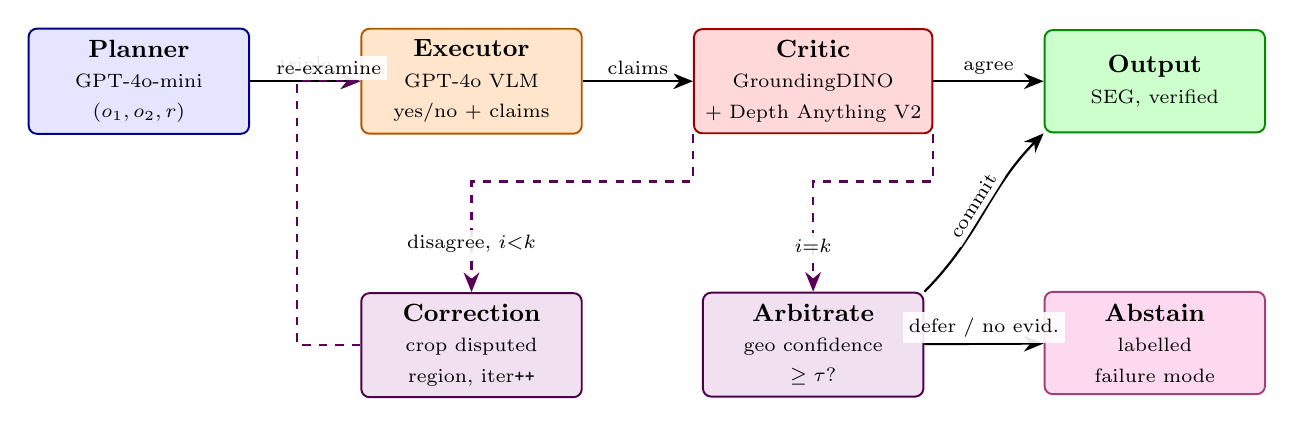
\begin{tikzpicture}[
  font=\small,
  >={Stealth[length=2.5mm,width=2mm]},
  node distance=10mm and 14mm,
  agent/.style={draw, rounded corners=3pt, align=center,
                minimum height=13mm, minimum width=28mm,
                inner xsep=4pt, inner ysep=4pt, line width=0.7pt},
  planner/.style={agent, fill=blue!10,    draw=blue!55!black},
  exec/.style   ={agent, fill=orange!20,  draw=orange!70!black},
  critic/.style ={agent, fill=red!15,     draw=red!60!black},
  ctrl/.style   ={agent, fill=violet!12,  draw=violet!60!black},
  outbox/.style ={agent, fill=green!20,   draw=green!55!black},
  abst/.style   ={agent, fill=magenta!15, draw=magenta!60!black},
  flow/.style={->, thick},
  loop/.style={->, thick, dashed, draw=violet!70!black},
  edgelbl/.style={font=\scriptsize, inner sep=2pt, fill=white, fill opacity=0.9, text opacity=1},
]

% Top row: linear pipeline
\node[planner] (P) {\textbf{Planner}\\\scriptsize GPT-4o-mini\\\scriptsize $(o_1,o_2,r)$};
\node[exec,    right=of P] (E) {\textbf{Executor}\\\scriptsize GPT-4o VLM\\\scriptsize yes/no + claims};
\node[critic,  right=of E] (C) {\textbf{Critic}\\\scriptsize GroundingDINO\\\scriptsize + Depth Anything V2};
\node[outbox,  right=of C] (O) {\textbf{Output}\\\scriptsize SEG, verified};

% Bottom row
\node[ctrl, below=20mm of E] (R) {\textbf{Correction}\\\scriptsize crop disputed\\\scriptsize region, iter\texttt{++}};
\node[ctrl, below=20mm of C] (A) {\textbf{Arbitrate}\\\scriptsize geo confidence\\\scriptsize $\geq\tau$?};
\node[abst, below=20mm of O] (X) {\textbf{Abstain}\\\scriptsize labelled\\\scriptsize failure mode};

% --- Happy path (solid) ---
\draw[flow] (P) -- node[edgelbl,above]{triple} (E);
\draw[flow] (E) -- node[edgelbl,above]{claims} (C);
\draw[flow] (C) -- node[edgelbl,above]{agree} (O);

% --- Correction loop: disagree, budget remaining (dashed, exits Critic SW) ---
\draw[loop] (C.south west) -- ++(0,-6mm) -| (R.north)
    node[edgelbl,pos=0.85,above]{disagree, $i{<}k$};
\draw[loop] (R.west) -- ++(-8mm,0) |- (E.west)
    node[edgelbl,pos=0.75,above]{re-examine};

% --- Arbitration: disagree, budget exhausted (dashed, exits Critic SE) ---
\draw[loop] (C.south east) -- ++(0,-6mm) -| (A.north)
    node[edgelbl,pos=0.85,above]{$i{=}k$};

% --- Arbitrate outputs (solid) ---
% commit: curve gracefully up and right to Output, well clear of Abstain
\draw[flow] (A.north east) to[out=45, in=225] node[edgelbl,sloped,above]{commit} (O.south west);
\draw[flow] (A) -- node[edgelbl,above]{defer / no evid.} (X);

\end{tikzpicture}
\caption{SEA pipeline. Three specialised agents communicate through a typed
\texttt{AgentState}. The correction loop zooms into the disputed region for up
to $k$ re-examinations; when the budget is exhausted, the arbitration node
commits geometry, defers to the VLM, or abstains based on geometric confidence.}
\label{fig:arch}
\end{figure*}

\section{Method}
SEA answers a binary spatial question $Q$ about image $I$ as follows.
\begin{enumerate}
\item \textbf{Parse.} The Planner converts $Q$ into a typed triple
$(\obj{obj}_1, \obj{obj}_2, r)$ with $r \in \mathcal{R} = \{$\rel{left\_of},
\rel{right\_of}, \rel{above}, \rel{below}, \rel{behind}, \rel{in\_front},
\rel{on}, \rel{contains}$\}$.
\item \textbf{Execute.} The Executor queries the VLM with $I$, the triple, and
a structured JSON prompt, returning an answer $\hat{a}\in\{$yes, no$\}$, a
confidence $c\in[0,1]$, and two object-claim strings.
\item \textbf{Verify.} The Critic detects $\obj{obj}_1, \obj{obj}_2$ with
GroundingDINO, estimates depth with Depth Anything V2, and applies the
deterministic rule for $r$ to produce a geometric verdict $v$ with a
\emph{geometric confidence} (Sec.~\ref{sec:recon}).
\item \textbf{Reconcile.} If $\hat{a}$ and $v$ agree, the answer is finalised
as \emph{verified}. If they disagree and $i<k$, the Critic crops the disputed
region (padding $\epsilon=0.05$) and re-examines. Otherwise the reconciliation
policy commits or abstains.
\item \textbf{Output.} The Output node assembles the SEG; on parse failure or
unrecoverable detector miss, the Abstain node records a labelled failure mode.
\end{enumerate}

\subsection{Spatial Predicate DSL}
All relations resolve to one of the eight deterministic rules in
Table~\ref{tab:dsl}. A slack threshold $\delta=0.02$ in normalised image
coordinates prevents spurious failures when objects are nearly aligned;
centroids $c_x, c_y$ and depths $d$ live in $[0,1]$.

\begin{table}[!htbp]
\centering
\small
\caption{Spatial Predicate DSL. Coordinates normalised to $[0,1]$.}
\label{tab:dsl}
\begin{tabular}{ll}
\toprule
Relation & Geometric rule \\
\midrule
\rel{left\_of}  & $c_x(o_1)-c_x(o_2) < -0.02$ \\
\rel{right\_of} & $c_x(o_1)-c_x(o_2) > +0.02$ \\
\rel{above}     & $c_y(o_1)-c_y(o_2) < -0.02$ \\
\rel{below}     & $c_y(o_1)-c_y(o_2) > +0.02$ \\
\rel{behind}    & $d(o_1)-d(o_2) > +0.02$ \\
\rel{in\_front} & $d(o_1)-d(o_2) < -0.02$ \\
\rel{on}        & $\Delta c_y < -0.02$ \textbf{and} IoU $> 0.05$ \\
\rel{contains}  & coverage $> 0.70$ \textbf{and} area ratio $< 0.70$ \\
\bottomrule
\end{tabular}
\end{table}

\subsection{Agents}
Figure~\ref{fig:arch} shows the pipeline. Each agent is a stateless LangGraph
node reading and writing a single typed \texttt{AgentState}, keeping all
inter-agent communication serialisable to JSON.

\textbf{Planner.} GPT-4o-mini converts the free-form question into the
structured triple using a strict system prompt encoding the eight-relation
DSL. It uses LangChain structured output when available and a JSON decoder
otherwise; a conservative regex fallback handles common phrasings if both
paths fail. Inverse phrasings (``inside'', ``within'') are normalised into the
\rel{contains} form by swapping the object order.

\textbf{Executor.} GPT-4o is queried with the image and a system prompt that
mandates a JSON record with an answer, a $0$--$1$ confidence, and two object
claims with visibility flags. The claims tell the Critic what to localise; the
confidence is later examined as a candidate abstention signal
(Sec.~\ref{sec:analysis}).

\textbf{Critic.} The Critic is the geometric engine. It detects both objects
with GroundingDINO using a dot-separated prompt, estimates a normalised depth
map with Depth Anything V2 Small, applies the DSL rule for the parsed
relation, and logs a \texttt{CriticEvidence} record. It never guesses: if
detection misses or the rule is indeterminate, the verdict is \emph{False} and
the failure is labelled.

\textbf{Correction.} The correction node is a deterministic state update, not
a learned agent: it increments the iteration counter and sets the crop region
the Critic computed around the disputed boxes, routing back to the Executor for
a re-run on the zoomed image.

\subsection{Depth in a Consistent Frame}
The active-perception loop re-examines a cropped region when the Executor and
Critic disagree. A subtle but important requirement is that depth values must
be \emph{comparable across iterations}. Depth Anything produces relative depth
normalised within its input image, so estimating depth on a cropped image and
comparing it to depth from the full image yields incommensurable values and
can flip \rel{behind}/\rel{in\_front} verdicts between iterations. SEA computes
depth once on the \emph{original} frame and samples it using the
original-frame bounding boxes (mapped back from crop coordinates), so depth
ordering is stable across the loop. On a held-out diagnostic set this
correction removed the observed depth oscillation, eliminated the
\texttt{depth\_noise} abstentions it caused, and reduced the mean correction
iterations from $1.33$ to $1.17$.

\subsection{Confidence-Based Reconciliation}
\label{sec:recon}
When the Executor and geometry still disagree after $k$ iterations, the
question is which signal to trust. We attach to each verification a
\emph{geometric confidence}
\begin{equation}
g = \min\!\big(\text{conf}(o_1),\text{conf}(o_2)\big)\cdot
\min\!\Big(1,\tfrac{|s|}{\sigma}\Big),
\end{equation}
the product of the two detector confidences and a margin-clearance term, where
$s$ is the deciding signal ($\Delta c_x$, $\Delta c_y$, $\Delta d$, or
coverage) and $\sigma$ a per-relation scale. Depth relations receive a smaller
scale and a confidence cap, encoding their unreliability; \rel{contains}
receives the same cap, for a reason the data forced on us. On VSR most
true-containment items have the reference object \emph{larger} than and barely
overlapping the container (captions whose boxes do not reflect visual nesting),
so the coverage/area signal is \emph{non-separable}: no threshold setting beats
3/12 true positives. We therefore cap \rel{contains} confidence so it defers to
the VLM rather than committing a verdict the geometry cannot support, which
removes the one relation on which SEA previously trailed the baseline.

The reconciliation policy is then: (i) if $g\ge\tau$ (default $0.40$),
\emph{commit the geometry verdict}; (ii) otherwise \emph{defer to the VLM};
(iii) if there is no usable geometric evidence (detector miss), either defer to
the VLM (full-coverage mode) or \emph{abstain} (selective mode). This replaces
a naive ``abstain on any disagreement'' rule and lets SEA act as a router that
sends each question to whichever signal is most trustworthy.

The per-relation scale $\sigma$ encodes a prior on signal reliability:
well-separated position relations (\rel{left\_of}, \rel{on}) clear the margin
decisively and earn high confidence, whereas depth relations (\rel{behind},
\rel{in\_front}) and \rel{contains} draw on noisier or non-separable signals
and are explicitly capped. Figure~\ref{fig:geoconf} shows the resulting
distribution: depth and \rel{contains} relations sit below the arbitration
threshold by design, so SEA defers them to the VLM rather than overruling it
--- a choice the data in Sec.~\ref{sec:analysis} validates.

\begin{figure}[!htbp]
\centering
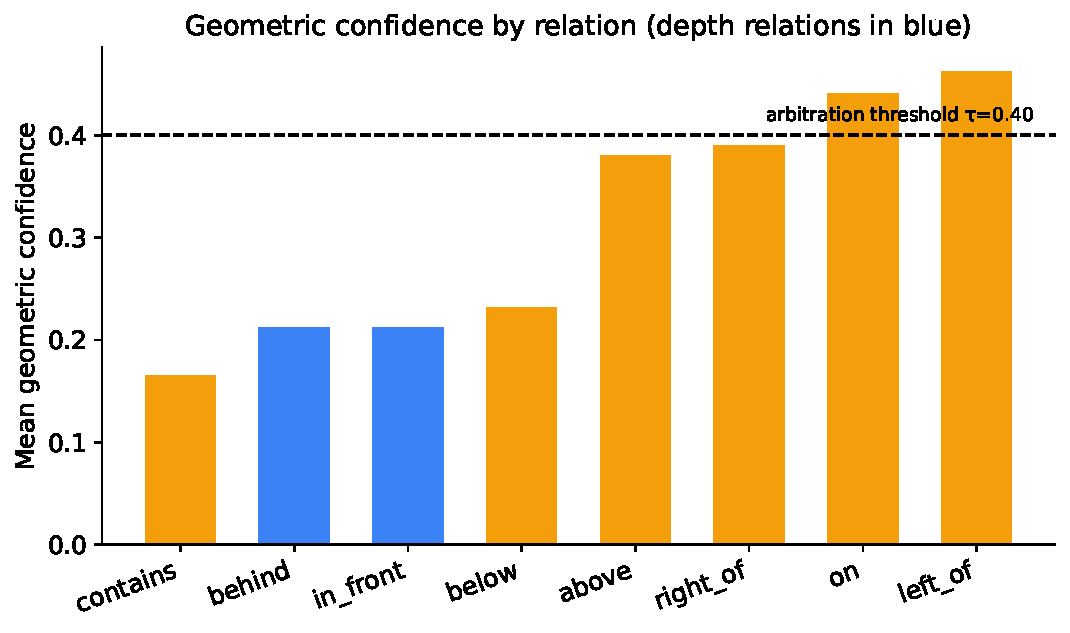
\includegraphics[width=\linewidth]{../results/figures/paper/paper_fig8_geoconf_by_relation.pdf}
\caption{Mean geometric confidence by relation. Depth relations (blue) and the
non-separable \rel{contains} relation fall below the arbitration threshold
$\tau=0.40$ and defer to the VLM; well-separated position relations clear it
and can commit geometry.}
\label{fig:geoconf}
\end{figure}

\subsection{Spatial Evidence Graph}
The SEG is a Pydantic-validated structure serialising the full trace: the
scene-graph triple, the final answer and its source
(\texttt{agreement}/\texttt{geometry\_override}/\texttt{vlm\_deferred}), a
confidence, and a list of \texttt{CriticEvidence} records storing raw boxes,
depths, centroid deltas, IoU, the applied rule, and any failure reason. Every
decision is thus auditable and reproducible.

\section{System and Implementation}
SEA is implemented as a LangGraph \texttt{StateGraph} in which every agent is
a pure function over a single Pydantic \texttt{AgentState}. Two routing
functions, \texttt{route\_after\_planner} and \texttt{route\_after\_critic},
encode the control flow: the former handles parse errors, the latter handles
agreement, disagreement-with-budget (route to \texttt{correction}), and
budget-exhausted disagreement (route to the confidence-based arbitration
node). This cleanly separates orchestration from agent logic and makes the
entire trace serialisable.

\textbf{Strict vs.\ permissive execution.} Production runs use a
\emph{strict} mode in which Planner or Executor model failures halt the query
rather than silently falling back, ensuring reported numbers reflect genuine
model behaviour. A permissive mode (regex Planner fallback, deterministic mock
detector/depth) supports offline testing without GPU or API access.

\textbf{Geometric configuration.} All thresholds --- the slack $\delta$, the
\rel{on}/\rel{contains} IoU and coverage cutoffs, the arbitration threshold
$\tau$, the depth-confidence cap, and the crop padding $\epsilon$ --- live in a
single typed configuration object, so an ablation or a deployment can retune
the geometry without touching agent code.

\textbf{Caching.} Because the correction loop revisits the same image, the
depth map is computed once per image on the original frame and memoised, while
detection is recomputed per crop. This keeps the active-perception loop cheap
and, as Sec.~\ref{sec:recon} describes, depth-frame consistent.

\textbf{Reproducibility.} The geometry engine is covered by a unit-test suite
exercising every predicate and the confidence computation on synthetic boxes,
plus an end-to-end pipeline smoke test. The VSR-200 split, the stratified
sampler, the evaluation harness, and the figure-generation scripts are all
deterministic given a fixed seed, so every table and figure in this report can
be regenerated from the released code.

\section{Experimental Setup}
\textbf{Dataset.} We evaluate on \textbf{VSR}~\cite{vsr}, a published binary
yes/no spatial-relation benchmark over COCO images. We build a
\emph{stratified 200-sample split} covering all eight relations our pipeline
supports (23--27 items each; 95 \emph{yes} / 105 \emph{no}). VSR's declarative
captions are converted to questions of the form ``Is the $\obj{obj}_1$ $r$ the
$\obj{obj}_2$?''; relations outside our DSL are filtered out. This scales
evaluation well beyond the 12-sample prototype used at the
mid-demonstration.

\textbf{Backend.} GPT-4o-mini Planner, GPT-4o Executor, GroundingDINO
SwinT-OGC and Depth Anything V2 Small Critic, on a single RTX~5090. The
correction loop uses $k=2$ unless noted.

\textbf{Baseline.} The \emph{executor-only} baseline runs the same Planner and
GPT-4o Executor but skips the Critic, taking the VLM's yes/no answer directly.
This isolates the contribution of geometric verification on identical images.

\textbf{Metrics.} Accuracy (over all items; abstentions count as wrong);
selective accuracy (over committed items only); coverage (fraction answered);
and answer-source attribution.

\section{Results}
\textbf{Main result.} Table~\ref{tab:main} reports the headline comparison. At
full coverage, SEA attains \textbf{79.0\%}, a \textbf{$+7.0$-point} gain over
the strong GPT-4o baseline (72.0\%). In selective mode --- abstaining only
when there is no geometric evidence --- SEA's committed answers reach
\textbf{80.3\% selective accuracy at 89.0\% coverage}, i.e.\ \emph{more
accurate than the VLM} while every answer carries explicit geometric evidence.
Figure~\ref{fig:headline} visualises both operating points.

\begin{table}[!htbp]
\centering
\small
\caption{Main results on the VSR-200 split. All SEA operating points exceed
the GPT-4o baseline on their respective metric. The high-precision row
abstains on roughly 70\% of items by design, so its full-denominator accuracy
is not the operative metric (omitted); its committed answers are 85\% correct.}
\label{tab:main}
\begin{tabular}{lccc}
\toprule
System & Acc. & Sel.\ acc. & Coverage \\
\midrule
GPT-4o baseline             & 0.720 & 0.720 & 1.000 \\
SEA (full coverage)         & \textbf{0.790} & 0.790 & 1.000 \\
SEA (selective)             & 0.715 & 0.803 & 0.890 \\
SEA (high precision, $\tau{=}0.40$) & --- & \textbf{0.847} & 0.295 \\
\bottomrule
\end{tabular}
\end{table}

\begin{figure}[!htbp]
\centering
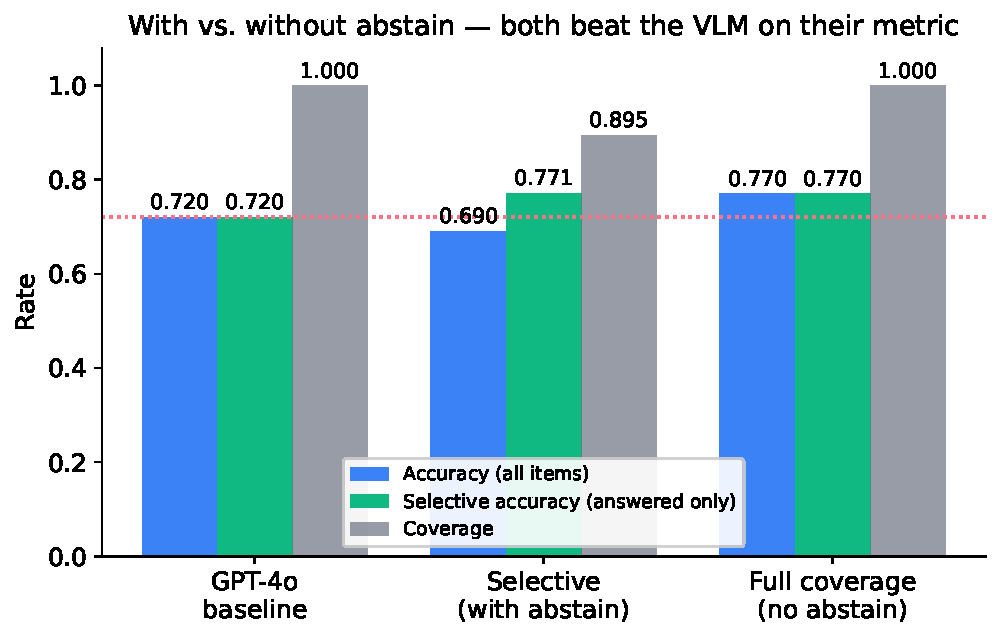
\includegraphics[width=\linewidth]{../results/figures/paper/paper_fig2_with_without_abstain.pdf}
\caption{SEA vs.\ the GPT-4o baseline. The full-coverage model improves raw
accuracy ($+7.0$ pts); the selective model exceeds the baseline in selective
accuracy while answering 89.0\% of items with verified evidence.}
\label{fig:headline}
\end{figure}

\textbf{Reconciliation-policy ablation.} Table~\ref{tab:ablation} shows that
the reconciliation policy is the main driver of accuracy. A naive
``abstain-on-disagreement'' rule sacrifices coverage without a precision gain;
adding confidence-based arbitration, then routing depth disagreements to the
VLM, then deferring detector-misses to the VLM monotonically improves
full-denominator accuracy to 0.77; a final geometry recalibration --- a wider
position slack and deferring the non-separable \rel{contains} relation
(Sec.~\ref{sec:recon}) --- lifts it to 0.79. Each design choice contributes,
confirming that the gain is policy-driven --- geometry is used to
\emph{route}, not to overrule.

\begin{table}[!htbp]
\centering
\small
\caption{Reconciliation-policy ablation (VSR-200, $k=2$). Each row adds one
design choice over the previous.}
\label{tab:ablation}
\begin{tabular}{lcc}
\toprule
Policy & Acc. & Coverage \\
\midrule
Abstain on disagreement        & 0.490 & 0.650 \\
\;+ confidence arbitration     & 0.655 & 0.895 \\
\;+ depth defers to VLM (sel.) & 0.690 & 0.895 \\
\;+ VLM fallback (full cov.)   & 0.770 & 1.000 \\
\;+ margin \& \rel{contains} recal. & \textbf{0.790} & 1.000 \\
\bottomrule
\end{tabular}
\end{table}

\begin{figure}[!htbp]
\centering
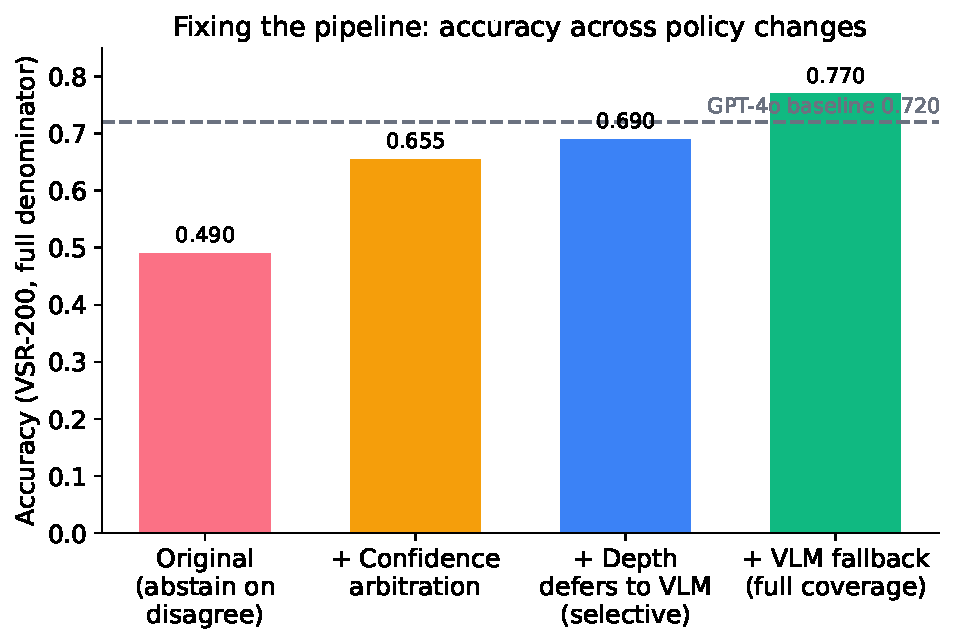
\includegraphics[width=\linewidth]{../results/figures/paper/paper_fig1_journey.pdf}
\caption{Accuracy across reconciliation-policy design steps. Each change moves
SEA upward; the final full-coverage policy crosses the GPT-4o baseline. The
gain is driven by how disagreements are reconciled, not by changing the
underlying detector or depth model.}
\label{fig:journey}
\end{figure}

\textbf{How answers are produced.} SEA behaves as a verifier and router rather
than a competing predictor. Table~\ref{tab:source} attributes committed
answers to their source: most items are \emph{agreements} between the Executor
and geometry, which are reliable; the rest are high-confidence geometry
commits or VLM deferrals. Every committed bucket answers at $\ge 0.80$,
confirming that the routing sends questions to a trustworthy signal.

\begin{table}[!htbp]
\centering
\small
\caption{Answer-source attribution (selective mode). Abstentions arise only
from detector misses.}
\label{tab:source}
\begin{tabular}{lcc}
\toprule
Source & $n$ & Accuracy \\
\midrule
agreement          & 138 & 0.80 \\
VLM deferred       & 34  & 0.82 \\
geometry override  & 6   & 0.83 \\
abstain (det.\ miss) & 22 & --- \\
\bottomrule
\end{tabular}
\end{table}

\textbf{Per-relation behaviour.} Figure~\ref{fig:perrel} compares SEA to the
baseline per relation. SEA improves most on relations where the baseline is
weakest --- notably \rel{in\_front} (0.83 vs 0.54) and \rel{right\_of} (0.92
vs 0.79) --- and, after recalibration, matches or exceeds the baseline on
\emph{every} relation, including \rel{contains}, where the
\rel{contains}-defer change removed the prior regression. (Per-relation counts
are $\sim$25, so individual entries are indicative rather than statistically
tight.)

\begin{figure}[!htbp]
\centering
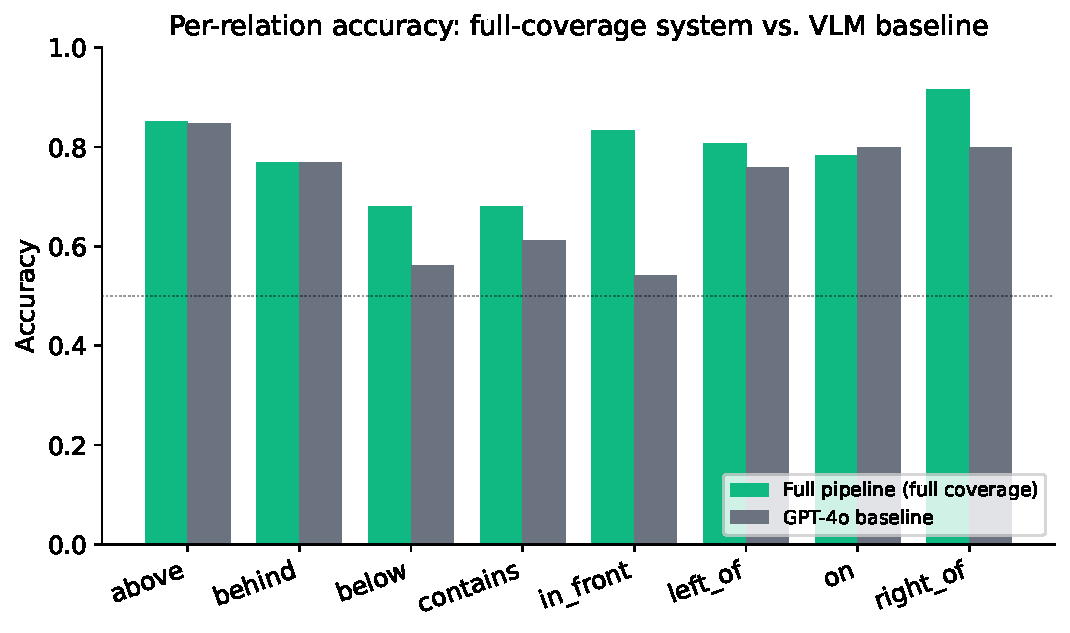
\includegraphics[width=\linewidth]{../results/figures/paper/paper_fig7_per_relation_final.pdf}
\caption{Per-relation accuracy, full-coverage SEA vs.\ GPT-4o baseline. SEA
improves markedly on \rel{in\_front} and \rel{right\_of} and matches or beats
the baseline on every relation.}
\label{fig:perrel}
\end{figure}

\textbf{Error structure.} Figure~\ref{fig:confusion} shows that, relative to
the baseline, SEA's gain comes chiefly from \emph{recovering true-positive
``yes'' answers}: it correctly confirms 10 more genuine spatial relations than
the VLM alone (69 vs.\ 59 true positives) at \emph{lower} false-positive cost
(16 vs.\ 20). Verification thus reduces the VLM's tendency to wrongly deny
relations that are in fact present.

\begin{figure}[!htbp]
\centering
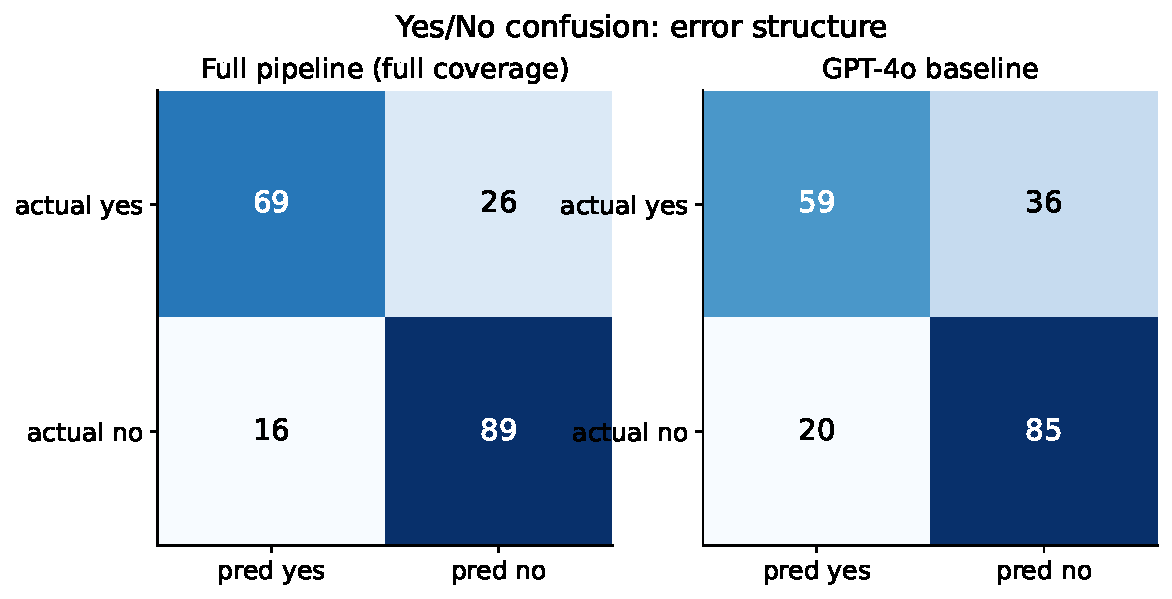
\includegraphics[width=\linewidth]{../results/figures/paper/paper_fig9_confusion.pdf}
\caption{Yes/No confusion. SEA (left) recovers 10 more true ``yes'' answers
than the baseline (right) at lower false-positive cost.}
\label{fig:confusion}
\end{figure}

\section{Analysis: Geometry as an Uncertainty Signal}
\label{sec:analysis}
A well-designed selective predictor should abstain on the items it is most
likely to get wrong, so accuracy on retained items rises as coverage falls. We
test which per-item signal best ranks errors by sorting items
most-confident-first and sweeping the abstain threshold
(Figure~\ref{fig:riskcov}).

\begin{figure}[!htbp]
\centering
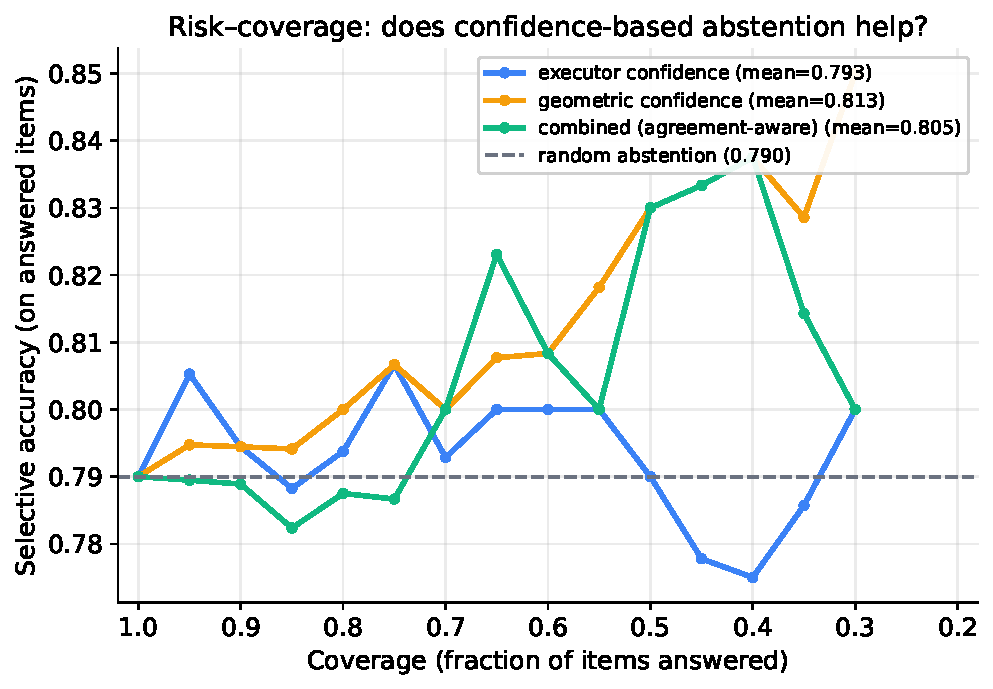
\includegraphics[width=\linewidth]{../results/figures/paper/paper_fig5_risk_coverage.pdf}
\caption{Risk--coverage. Sorting by geometric confidence and abstaining on the
least-confident items raises selective accuracy well above random abstention;
the VLM's own confidence is far less informative.}
\label{fig:riskcov}
\end{figure}

Two findings emerge. First, the VLM's self-reported confidence is nearly
useless for selective prediction: it occupies a narrow $0.80$--$1.00$ band
(mean $0.91$) and ranks errors barely above chance
(Figure~\ref{fig:inform}, right). Second, \textbf{geometric confidence is a
genuinely informative uncertainty signal}: abstaining on low-geometric-
confidence items lifts selective accuracy toward $0.85$
(Figure~\ref{fig:inform}, left). This holds even though geometry is a weaker
\emph{answer} source than the VLM --- the Critic knows \emph{when} the VLM is
likely wrong without itself answering better. It reframes the role of
deterministic geometry in VLM pipelines: its value is verification and
calibrated confidence, not raw answer accuracy.

\begin{figure}[!htbp]
\centering
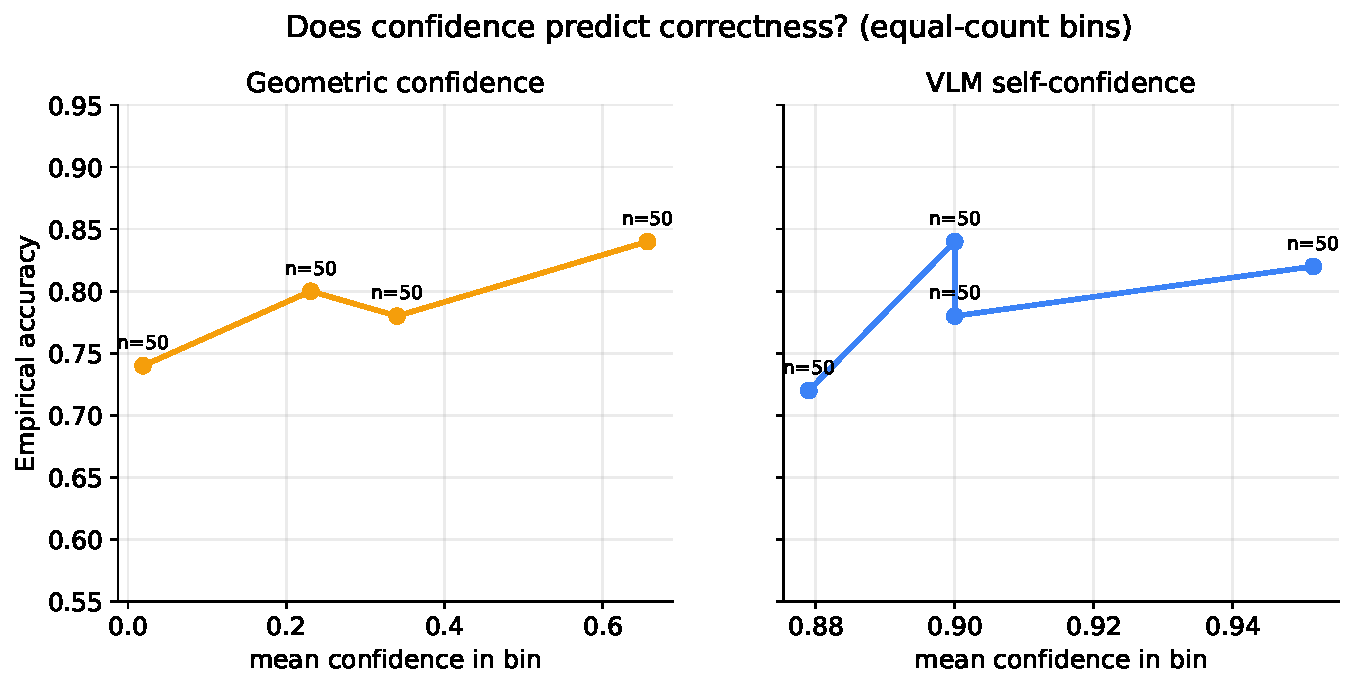
\includegraphics[width=\linewidth]{../results/figures/paper/paper_fig6_confidence_informativeness.pdf}
\caption{Empirical accuracy vs.\ confidence bin. Geometric confidence (left)
predicts correctness; the VLM's self-confidence (right) is compressed near
$1.0$ and far less discriminative.}
\label{fig:inform}
\end{figure}

This result directly informs system design. Because geometric confidence
ranks errors, it serves double duty: as the arbitration signal that decides
override-vs-defer (Sec.~\ref{sec:recon}), and as a tunable abstention signal
that exposes the precision/coverage frontier in Figure~\ref{fig:riskcov}. A
practitioner can therefore dial SEA to any desired operating point --- from
full coverage at $79.0\%$ to higher-precision selective regimes --- using a
single threshold, with the chosen point always accompanied by auditable
geometric evidence. Concretely, thresholding committed answers at
$\tau=0.40$ yields a verified \textbf{0.847 selective accuracy at 29.5\%
coverage} (Table~\ref{tab:main}) --- a $+13$-point precision gain over the
bare VLM, for applications where declining to answer beats a likely error.
Figure~\ref{fig:oppoints} places our reported configurations and the bare-VLM
baseline in the coverage/accuracy plane: all SEA points dominate the baseline,
and lowering coverage along the geometric-confidence threshold trades coverage
for verified, higher-precision answers.

\begin{figure}[!htbp]
\centering
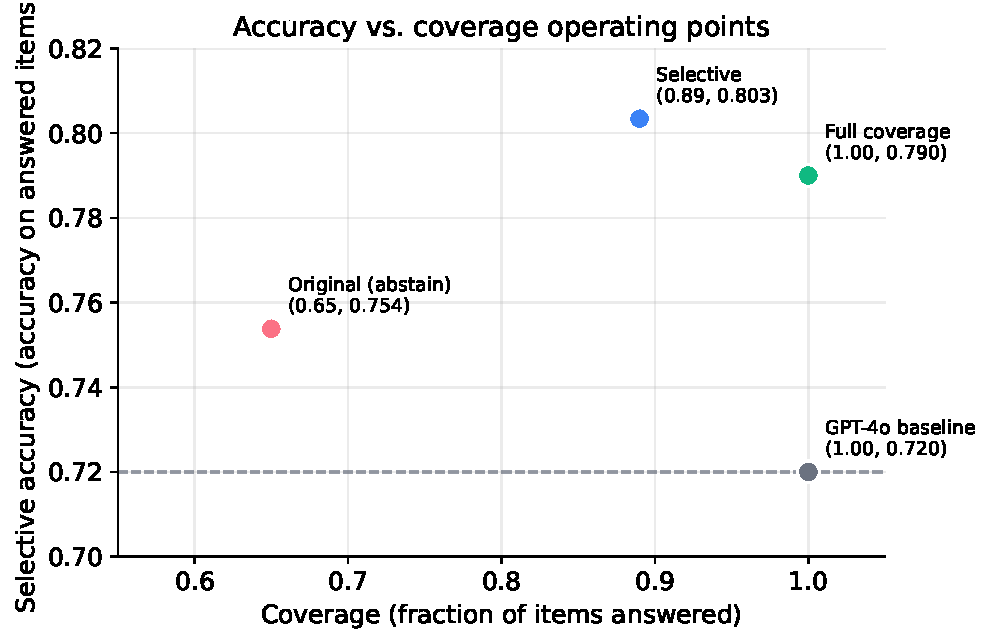
\includegraphics[width=\linewidth]{../results/figures/paper/paper_fig4_accuracy_vs_coverage.pdf}
\caption{Operating points in the coverage/accuracy plane. Both SEA
configurations sit above the GPT-4o baseline; the selective point answers
89.0\% of items at higher selective accuracy.}
\label{fig:oppoints}
\end{figure}

\section{Qualitative Results}
Figure~\ref{fig:qual} shows six outputs spanning the rule families. Row~1
collects verified positives across position and containment relations
(\rel{left\_of}, \rel{above}, \rel{contains}); row~2 covers the three depth
modes the system supports: \rel{in\_front} and \rel{behind} verify when the
$|\Delta d|$ margin is clear, while the bus/car case abstains when it is
not --- mirroring the policy of Sec.~\ref{sec:recon}.

\begin{figure}[!htbp]
\centering
\begin{subfigure}[t]{0.32\linewidth}
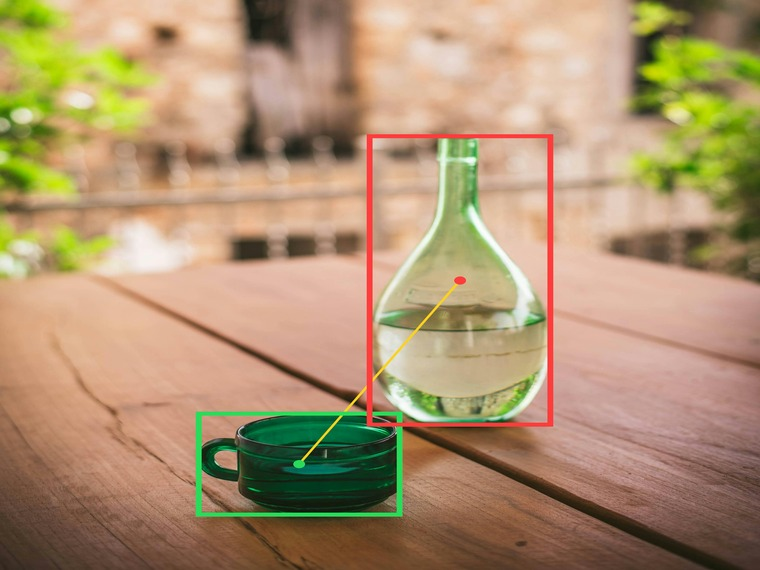
\includegraphics[width=\linewidth]{../results/figures/qual_panel_1.jpg}
\caption{\scriptsize \rel{left\_of}, verified}
\end{subfigure}\hfill
\begin{subfigure}[t]{0.32\linewidth}
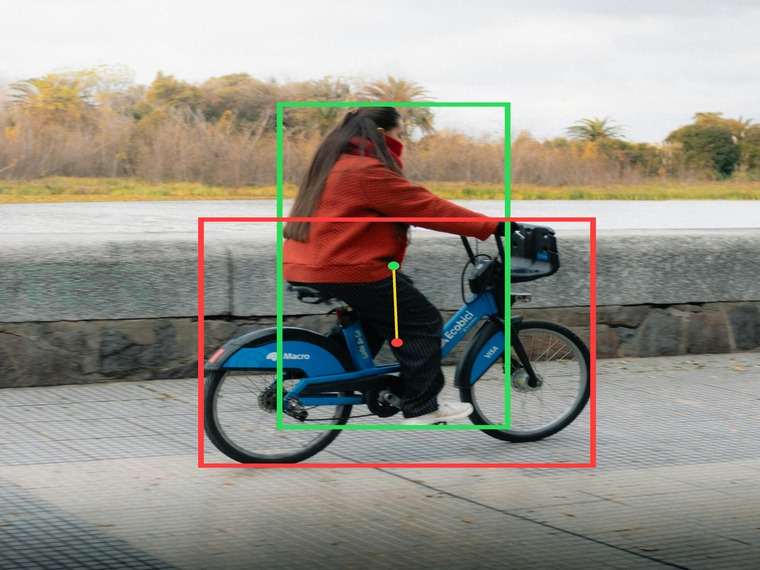
\includegraphics[width=\linewidth]{../results/figures/qual_panel_3.jpg}
\caption{\scriptsize \rel{above}, verified}
\end{subfigure}\hfill
\begin{subfigure}[t]{0.32\linewidth}
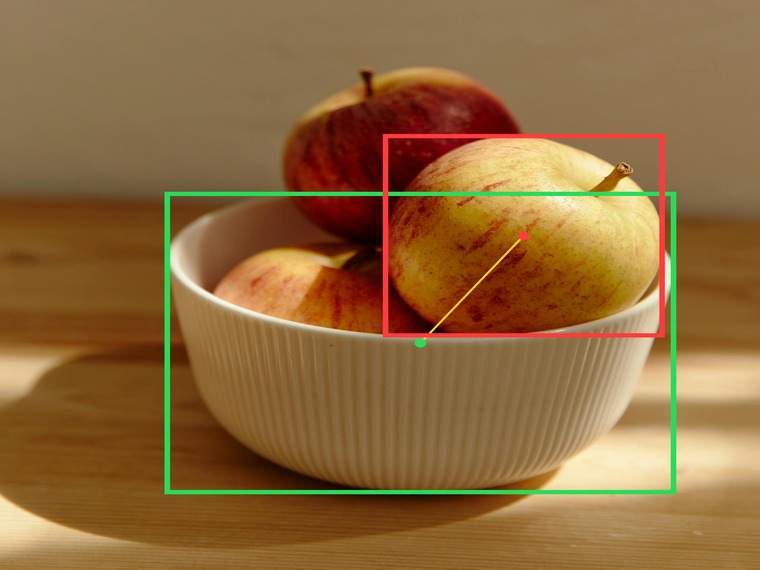
\includegraphics[width=\linewidth]{../results/figures/qual_panel_5.jpg}
\caption{\scriptsize \rel{contains}, verified}
\end{subfigure}

\vspace{1mm}

\begin{subfigure}[t]{0.32\linewidth}
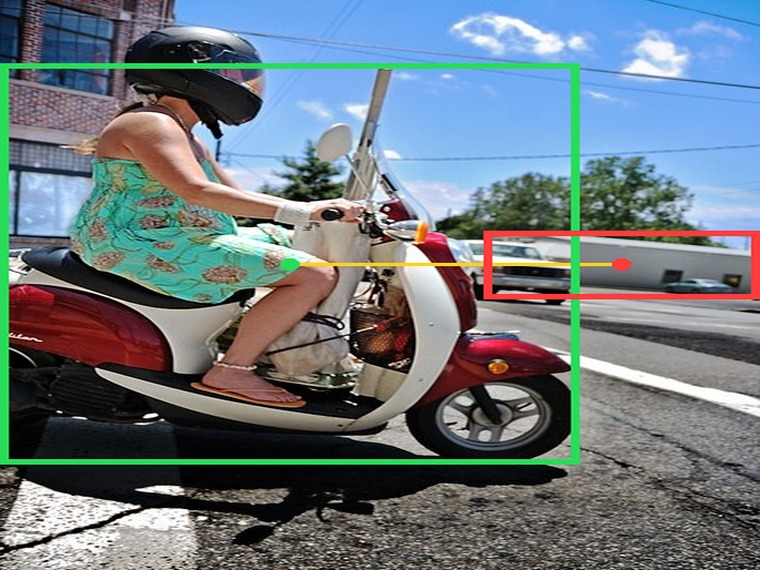
\includegraphics[width=\linewidth]{../results/figures/qual_panel_7.jpg}
\caption{\scriptsize \rel{in\_front}, verified}
\end{subfigure}\hfill
\begin{subfigure}[t]{0.32\linewidth}
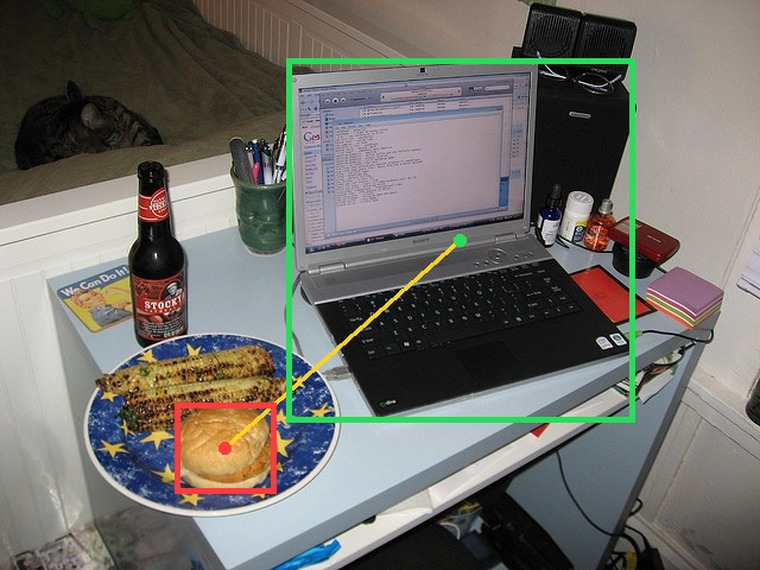
\includegraphics[width=\linewidth]{../results/figures/qual_panel_8.jpg}
\caption{\scriptsize \rel{behind}, verified}
\end{subfigure}\hfill
\begin{subfigure}[t]{0.32\linewidth}
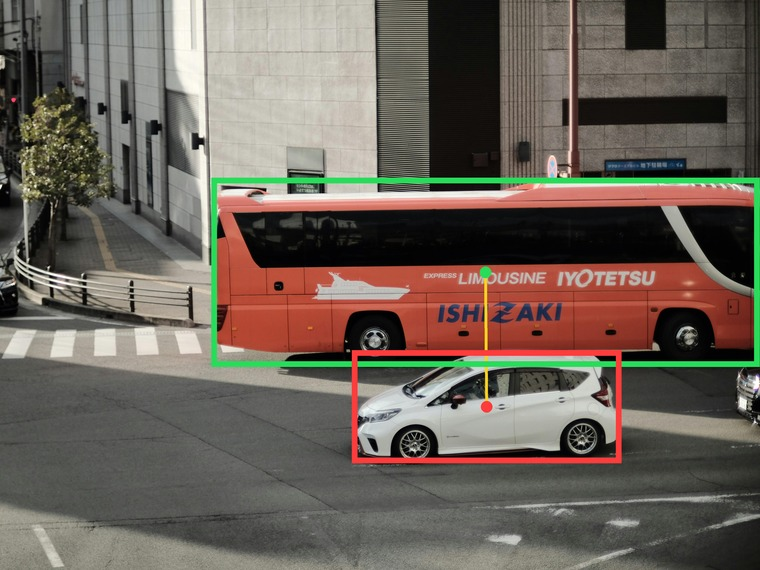
\includegraphics[width=\linewidth]{../results/figures/qual_panel_9.jpg}
\caption{\scriptsize \rel{behind}, abstained}
\end{subfigure}
\caption{Annotated outputs on six distinct scenes. Green/red boxes are
GroundingDINO detections for $\obj{obj}_1$/$\obj{obj}_2$; the applied rule and
its value are stored in the SEG. Row~1: verified positives on position and
containment. Row~2: depth verifies cleanly when the margin is large; on the
bus/car case the system abstains.}
\label{fig:qual}
\end{figure}

\textbf{Where geometry corrects the VLM.} Of the 200 items, SEA at full
coverage answers correctly on 22 questions on which the GPT-4o baseline is
wrong. Figure~\ref{fig:wins} shows three such cases, all decided by the
geometric \emph{override} path. In (a) and (b), GPT-4o misses a true relation
that a clean centroid margin makes obvious; in (c), GPT-4o asserts a relation
that geometry refuses --- the centroid ordering is inconsistent with
\rel{right\_of}, so the Critic flips the verdict to \emph{no}. These are
exactly the cases the confidence-based reconciliation policy is designed to
catch: when a strong geometric signal disagrees with the VLM, deferring to the
detector pays off.

\begin{figure}[!htbp]
\centering
\begin{subfigure}[t]{0.32\linewidth}
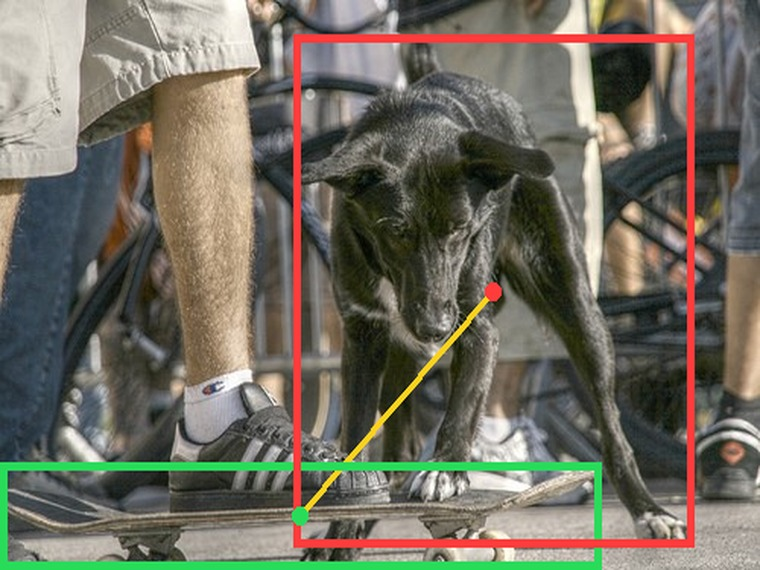
\includegraphics[width=\linewidth]{../results/figures/sea_vs_baseline_1.jpg}
\caption{\scriptsize \rel{left\_of}, skateboard/dog\\ GT yes \quad VLM $\times$ \quad SEA $\checkmark$}
\end{subfigure}\hfill
\begin{subfigure}[t]{0.32\linewidth}
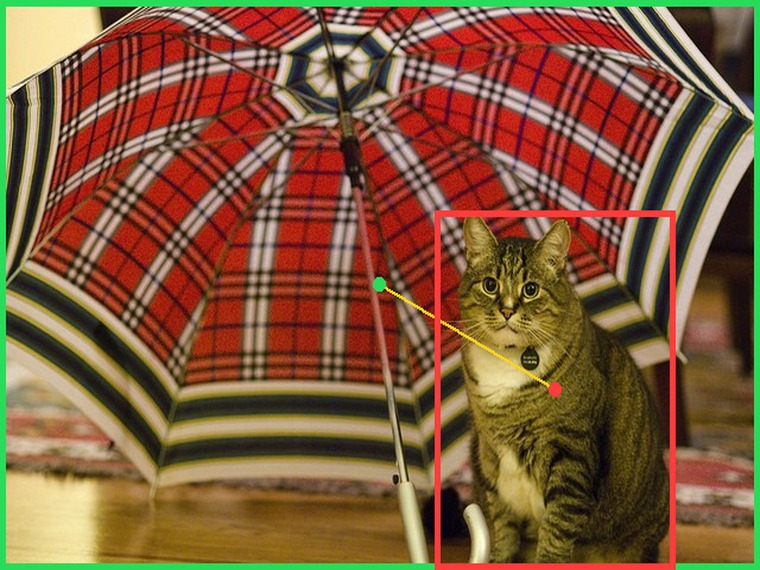
\includegraphics[width=\linewidth]{../results/figures/sea_vs_baseline_2.jpg}
\caption{\scriptsize \rel{above}, umbrella/cat\\ GT yes \quad VLM $\times$ \quad SEA $\checkmark$}
\end{subfigure}\hfill
\begin{subfigure}[t]{0.32\linewidth}
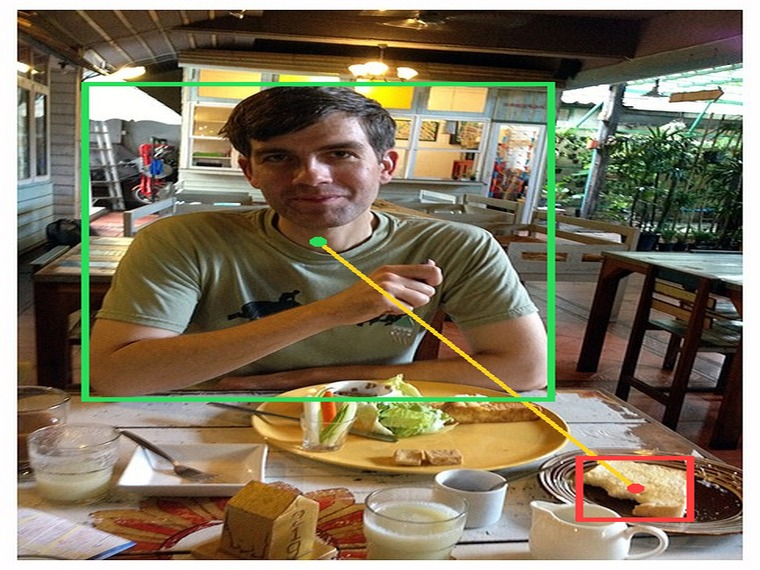
\includegraphics[width=\linewidth]{../results/figures/sea_vs_baseline_3.jpg}
\caption{\scriptsize \rel{right\_of}, person/cake\\ GT no \quad VLM $\times$ \quad SEA $\checkmark$}
\end{subfigure}
\caption{Cases where the GPT-4o baseline is wrong but SEA is right via the
geometric override path. (a, b) recover true positives the VLM missed;
(c) refuses a hallucinated positive when the centroid ordering contradicts the
relation.}
\label{fig:wins}
\end{figure}

\section{Discussion}
Our results invite a reinterpretation of how deterministic perception modules
should be combined with strong VLMs. The intuitive hope --- that closed-form
geometry can \emph{correct} a VLM's spatial mistakes --- holds only weakly:
when high-confidence monocular geometry contradicts GPT-4o, the VLM is usually
the more reliable party, particularly on depth. Overriding the VLM on such
disagreements is therefore counterproductive, which is precisely why SEA's
reconciliation policy defers depth disagreements rather than overruling them.

What geometry \emph{does} provide is a trustworthy, model-independent estimate
of \emph{when} a spatial answer is safe. Detector confidence and rule-margin
clearance jointly form a signal that ranks errors far better than the VLM's
own (badly calibrated) confidence. SEA exploits this in two ways: agreement
between the two independent estimators is a strong correctness cue (hence the
high accuracy of the \emph{agreement} bucket), and the geometric-confidence
score gives a continuous knob for selective prediction. The net effect is a
system that is both more accurate than the bare VLM at full coverage and fully
auditable --- every answer is accompanied by the boxes, depths, and rule
evaluation that produced it.

This view generalises beyond spatial VQA. Any setting in which a strong but
opaque generative model is paired with a weaker but transparent verifier can
benefit from the same recipe: rather than forcing the verifier to overrule the
generator, use the verifier's agreement and confidence to \emph{route} and to
\emph{abstain}. The transparency is not free --- it costs the extra detection
and depth passes --- but it converts an unaccountable black-box answer into one
backed by inspectable evidence, which is precisely what safety-sensitive
deployments require.

\textbf{Future work.} Three directions follow directly from our analysis.
First, replacing relative monocular depth with a metric estimator would let the
Critic safely \emph{correct} the VLM on depth relations rather than only defer,
potentially lifting the \rel{behind}/\rel{in\_front} ceiling. Second, because
geometric confidence is a calibrated error signal, an abstention threshold can
be \emph{learned} on held-out data to target a desired precision, replacing the
hand-set $\tau$. Third, passing VSR's reference-frame annotation to the Planner
would let SEA distinguish camera-relative from object-relative left/right
queries, removing a known source of position-relation error. Finally, scaling
the evaluation to the full VSR test set and to controlled benchmarks such as
WhatsUp~\cite{whatsup} would tighten the per-relation comparisons that are
currently estimated at $\sim$25 samples each.

\section{Limitations}
\textbf{Monocular depth.} Relative single-image depth remains the weakest
signal; SEA mitigates this by deferring depth disagreements to the VLM rather
than overriding them, but metric depth would enable genuine geometric
correction of depth relations.
\textbf{Scale.} VSR-200 covers COCO scenes with $\sim$25 items per relation;
per-relation comparisons are indicative, and broader evaluation across domains
is future work.
\textbf{Reference frame.} VSR mixes camera-relative and object-relative
framings for left/right; SEA assumes the camera frame, accounting for some
residual position-relation errors.
\textbf{Threshold calibration.} The position slack and the \rel{contains}
confidence cap were set on the same VSR-200 split we report on, using offline
replay of the dumped geometric evidence (no additional model calls). The
changes are principled --- the false-positive curve is monotone in the slack
and the \rel{contains} signal is provably non-separable --- but the absolute
gain is an in-distribution calibration result; held-out cross-split validation
is future work.
\textbf{Inference cost.} SEA issues a Planner call, one or more Executor
calls, and up to $k$ local Critic passes per query, versus a single VLM call
for the baseline; the full VSR-200 evaluation cost a few US dollars in API
spend plus GPU time for detection and depth. SEA is therefore best suited to
settings where verifiability and reliability outweigh per-query cost, rather
than latency-critical real-time use.

\section{Conclusion}
We presented the Spatial Evidence Agent, a training-free three-agent pipeline
that fuses VLM querying with deterministic geometric verification and a
confidence-based reconciliation policy. On a 200-sample VSR split SEA reaches
79.0\% accuracy at full coverage ($+7.0$ over a GPT-4o baseline) and 80.3\%
selective accuracy at 89.0\% coverage with fully auditable evidence. Our
analysis shows that the contribution of deterministic geometry is best
understood as \emph{verification and uncertainty estimation}: geometric
confidence reliably indicates when a VLM's spatial answer is trustworthy, even
where geometry alone is a weaker answerer. Future work includes metric-depth
integration, reference-frame-aware predicates, and learned, calibrated
abstention thresholds derived from the geometric-confidence signal.

\begin{thebibliography}{9}
\small
\bibitem{langgraph} LangChain, Inc. \emph{LangGraph: Building stateful,
multi-actor applications with LLMs.} 2024.
\bibitem{llava} H. Liu, C. Li, Q. Wu, Y. J. Lee. Visual instruction tuning.
\emph{NeurIPS}, 2023.
\bibitem{gdino} S. Liu et al. Grounding DINO: Marrying DINO with grounded
pre-training for open-set object detection. 2023.
\bibitem{depthanything} L. Yang et al. Depth Anything V2.
\emph{arXiv:2406.09414}, 2024.
\bibitem{whatsup} A. Kamath, S. Hessel, Y. Choi. What's ``up'' with
vision-language models? \emph{EMNLP}, 2023.
\bibitem{vsr} Z. Liu et al. Visual spatial reasoning. \emph{TACL}, 2023.
\bibitem{selective} Y. Geifman, R. El-Yaniv. Selective prediction in deep
neural networks. \emph{NeurIPS}, 2017.
\end{thebibliography}

\end{document}
